\section{Example}
As an exemplary scenario we take a look at the 13-dimensional UVB system and the 
\textsf{greedyseeds}. You can find the R notation of systems equations, observation function 
and a data set in the package. 
\begin{figure}[h]
\centering
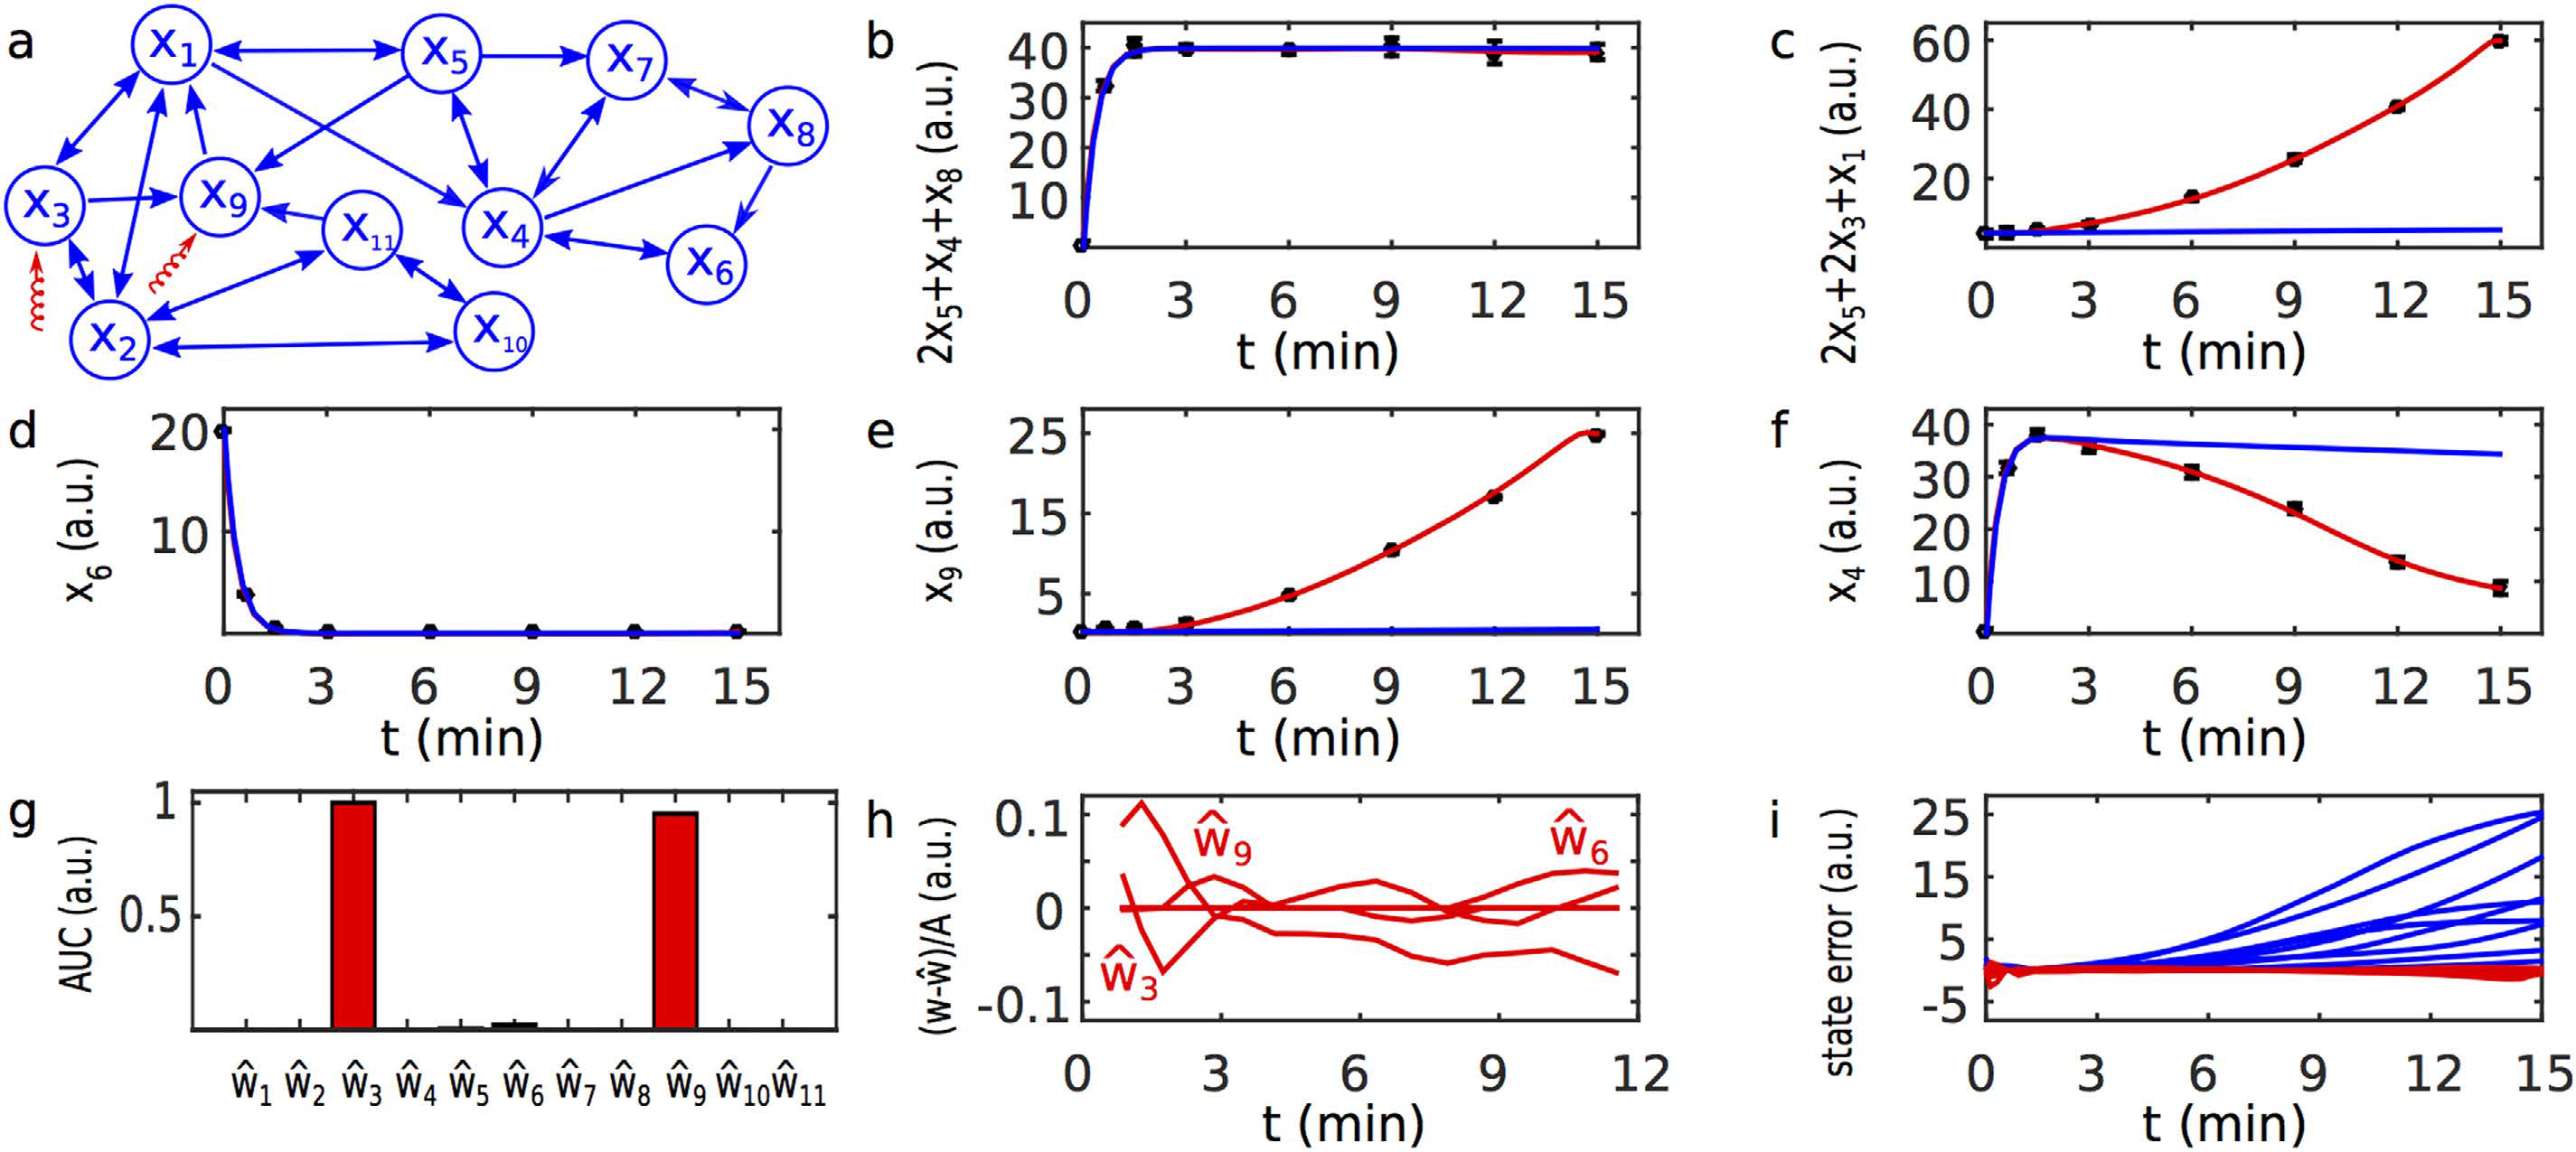
\includegraphics[scale=0.12]{figures/uvb.png}
\caption{Results of the \textsf{greedyseeds} algorithm. The black markers represent 
the data $y^\text{obs}$, the blue lines represent the erroneous model predictions and 
the red lines show the predictions using the estimated unknown inputs $\hat{w}_i$.}
\label{fig:example}
\end{figure}
Figure \ref{fig:example} shows the data and the five observables with erroneous system
predictions as black markers and blue lines, respectively. It also shows the estimated unknown 
inputs $\hat{w}_i$, the Area-Under-Curves and the predictions of the corrected model in red.
You see that the algorithm results in a sparse set of unknown inputs and how the unknown 
inputs are able to correct the model predictions such that these fit the data.